\documentclass[12pt]{article}
\usepackage[utf8]{inputenc}
\usepackage{amsmath}
\usepackage{graphicx}
\title{ Reporte de Producto 3}
\date{}
\begin{document}
  \maketitle
  En la práctica realizada el pasado martes durante las horas de laboratorio, corregimos y editamos ciertos programas hechos en lenguaje Fortran 90 para calcular áreas y volúmenes, entre otras cosas.
  A continuación se presenta un resumen de lo que se hizo en cada programa y se muestra evidencia de su correcto funcionamiento.\\
  
  1.  Programa Area.f90, para calcular el área de un círculo.\\
  Se corrigieron ciertos elementos de este programa, como los asteriscos y guiones bajos. Una vez realizada la corrección de la sintaxis, se obtuvo un programa resultante en el cual se introduce un radio para calcular su área.\\
\begin{verbatim}
 ! Area . f90 : Calculates the area of a circle, sample program
 ! −−−−−−−−−−−−−−−−−−−−−−−−−−−−−−−−−−−−−−−−−−−−−−−
 Program Circle_area ! Begin main program
  Implicit None ! Declare all variables
   Real *8 :: radius , circum , area ! Declare Reals
   Real *8 :: PI = 4.0 * atan(1.0) ! Declare , assign Real
  Integer :: model_n = 1 ! Declare , assign Ints
   print * , 'Enter a radius:' ! Talk to user
   read * , radius ! Read into radius
  Circum = 2.0 * PI * radius ! Calc circumference
  Area = radius * radius * PI ! Calc area
  print * , 'Program number =' , model_n ! Print program number
  print * , 'Radius =' , radius ! Print radius
  print * , 'Circumference =' , circum ! Print circumference
  print * , 'Area =' , area ! Print area
 End Program Circle_area ! End main program code
\end{verbatim}
 \begin{center}
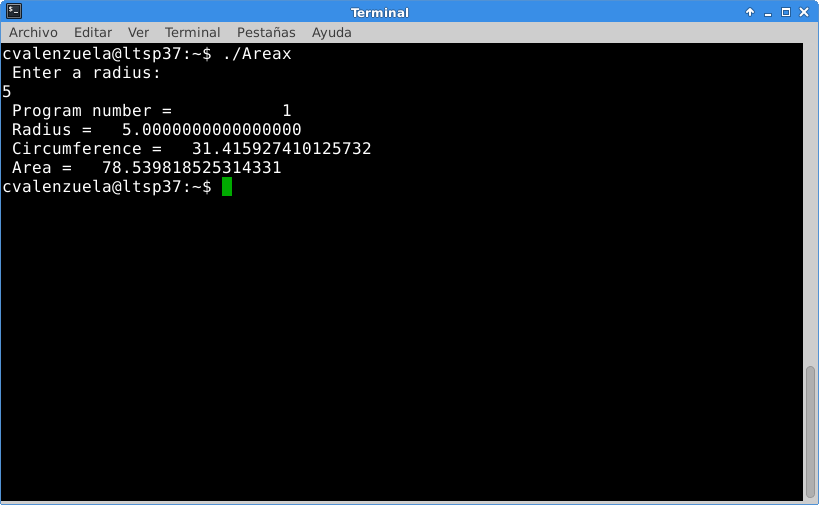
\includegraphics[width=0.5cm]{Area.png}\\
 \end{center}
  
  2.  Modifica el programa Area.f90 y crea un nuevo programa fuente Volumen.f90.\\
  Este nuevo programa derivado del primero, sirve para calcular el volumen que ocupa el líquido dentro de una esfera cuando se encuentra a una altura H.
  Se requirió modificar las dimensiones que el programa pide al usuario, así como la fórmula utilizada, siendo reemplazada la de área por volumen. Esta se tomó de referencia de la página proporcionada por el profesor.\\
  \begin{verbatim}
  ! Area . f90 : Calcular el volumen de liquido en un tanque esferico
 ! −−−−−−−−−−−−−−−−−−−−−−−−−−−−−−−−−−−−−−−−−−−−−−−
 Program Sphere_volume ! Begin main program
  Implicit None ! Declare all variables
   Real *8 :: radius , height , volume , Newradius ! Declare Reals
   Real *8 :: PI = 4.0 * atan(1.0) ! Declare , assign Real
  Integer :: model_n = 1 ! Declare , assign Ints
   print * , 'Enter a radius:' ! Talk to user
   read * , radius ! Read into radius
   print * , 'Enter a height:' ! Talk to user
   read * , height ! Tomar el valor de la h
   Newradius =  3 * radius - height  ! Calc volume
   volume = 0.3333 * PI * height * height * Newradius
 print * , 'Program number =' , model_n ! Print program number
  print * , 'Radius =' , radius ! Print radius
  print * , 'height =' , height ! Print height
  print * , 'Nuevo radio =' , Newradius
  print * , 'PI = ' , PI
  print * , 'Volume =' , volume ! Print circumference
 End Program Sphere_volume ! End main program code
 \end{verbatim}
  \begin{center}
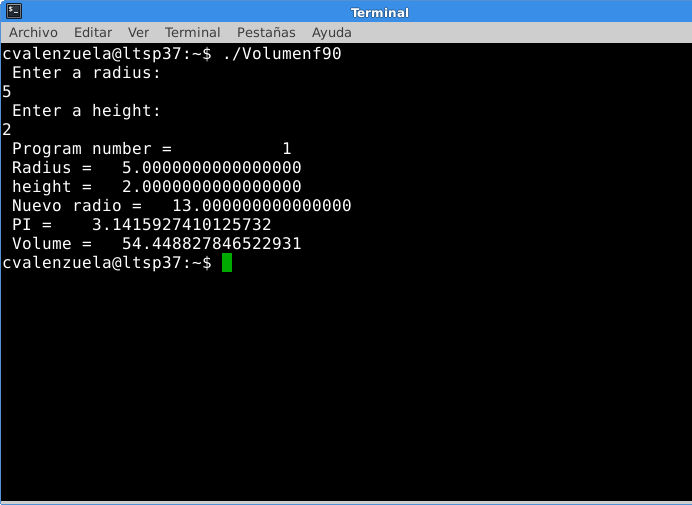
\includegraphics[width=0.5cm]{Volumenf90.png}\\
 \end{center}
  
  3. Determinando la precisión de la máquina.\\
  Este programa calcula la precisión de una máquina a manera de límite. Esta aproximación sugiere 8 cifras reales, por lo que se considera una precisión muy buena.Se modificaron algunos caracteres para obtener la sintaxis correcta para su compilación y corrimiento.\\
  \begin{verbatim}
  ! Limits . f90 : Determines machine precision
! LOOP, calculate each step and print .
 ! This loop will execute 60 times in a row as i is
 ! incremented from 1 to n ( since n = 60) :


 do i = 1, n , 1 ! Begin the docalculate one
   print * , i , one , epsilon_m ! Print values so far
 end do ! End loop when i>n
End Program Limits
 \end{verbatim}
  \begin{center}
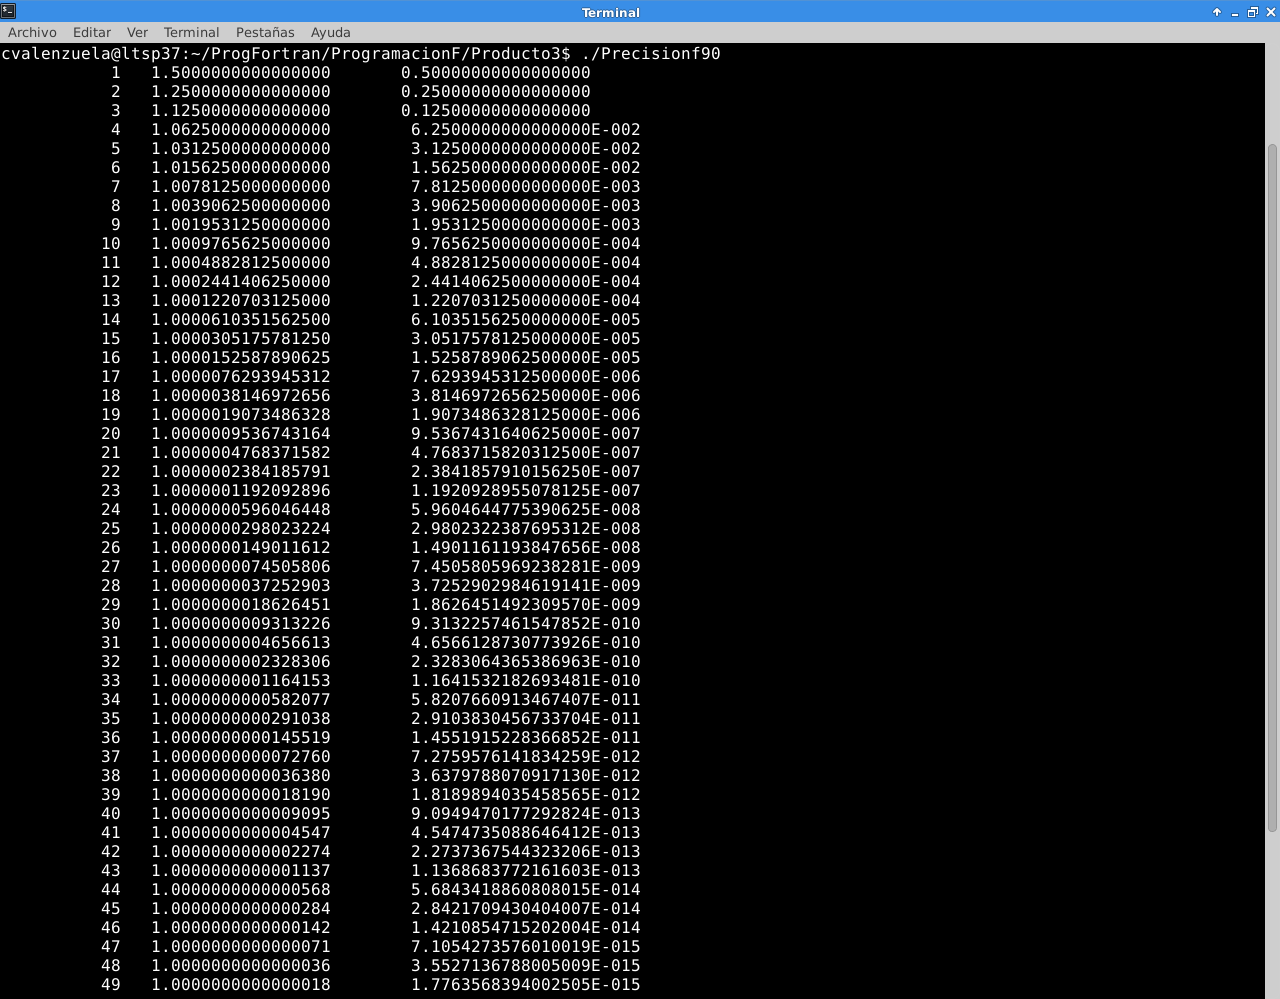
\includegraphics[width=0.5cm]{Precisionf90.png}\\
 \end{center}
 
 4. Modifica el programa anterior para realizar las operaciones en precisión sencilla: real *4 o simplemente real.\\
  Solo se cambió la leyenda "Real *8" por "Real *4", lo cual nos dio una aproximación un poco más burda.\\
  \begin{verbatim}
  ! Limits . f90 : Determines machine precision
! LOOP, calculate each step and print .
 ! This loop will execute 60 times in a row as i is
 ! incremented from 1 to n ( since n = 60) :


 do i = 1, n , 1 ! Begin the docalculate one
   print * , i , one , epsilon_m ! Print values so far
 end do ! End loop when i>n
End Program Real4
 \end{verbatim}
  \begin{center}
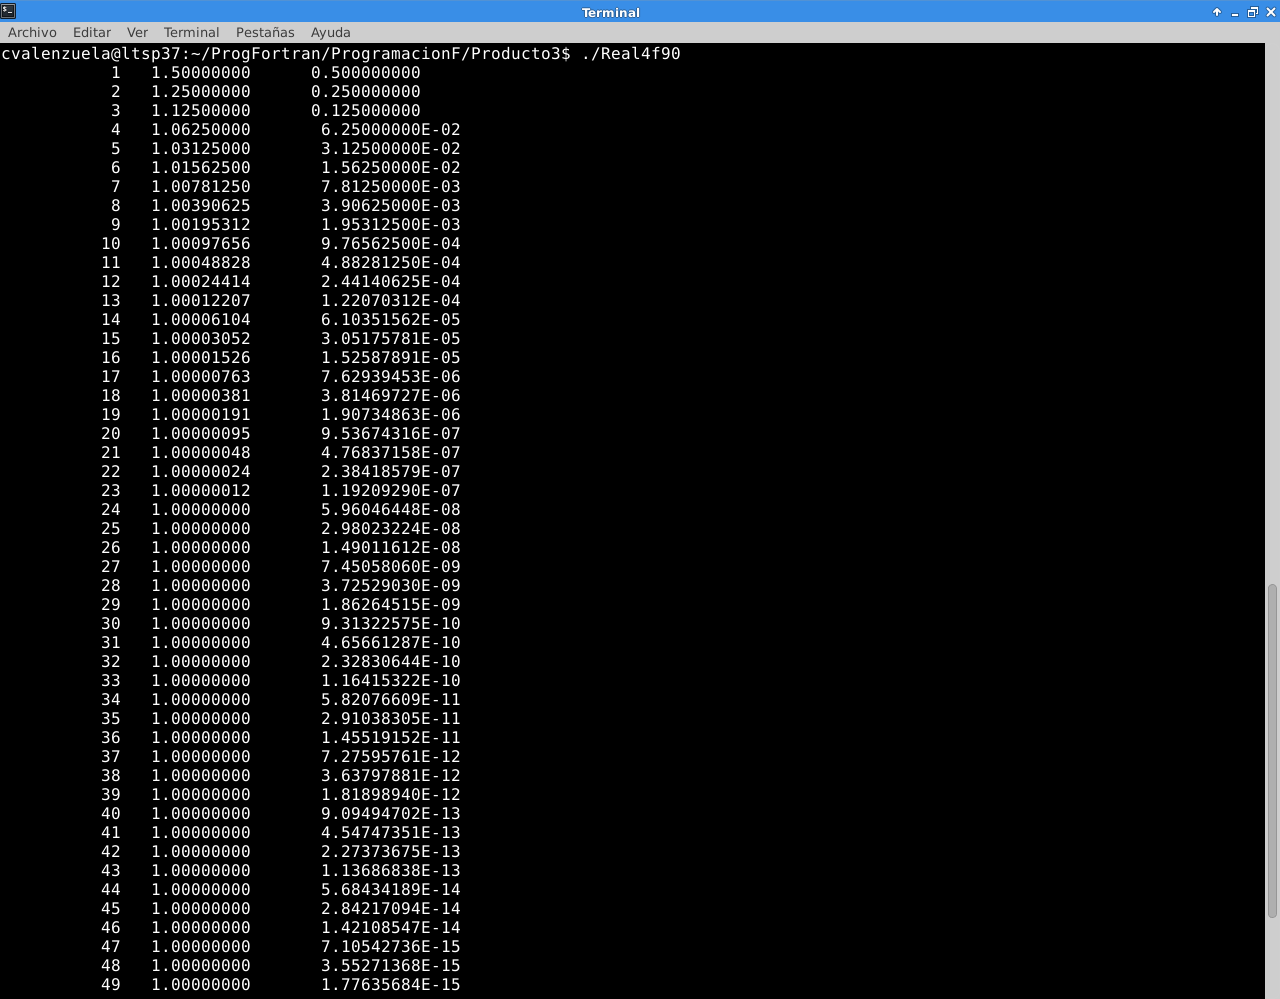
\includegraphics[width=0.5cm]{Real4f90.png}\\
 \end{center}
  
  5. Funciones trigonométricas.\\
  Sirve para calcular el seno y el valor de la función exponencial de las variables establecidas por el mismo programa. Se modificaron caracteres para la obtención de una correcta sintaxis.\\
  \begin{verbatim}
  ! Math . f90 : demo some Fortran math functions
!
Program Mathtest! Begin main program


  Real *8 :: x = 1.0 , y, z ! Declare variables x, y, z
  y = sin (x) ! Call the sine function
 z = exp (x) + 1.0 ! Call the exponential function
 print * , x, y, z ! Print x, y, z
End Program Mathtest ! End main program
 \end{verbatim}
  \begin{center}
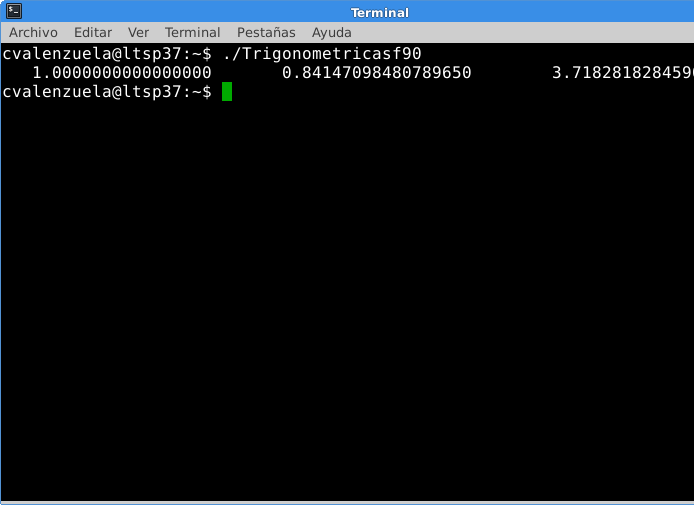
\includegraphics[width=0.5cm]{Trigonometricas.png}\\
 \end{center}
  6.  Modifica el programa anterior Math.f90\\
  Esto con el fin de obtener un nuevo programa que calcule la raíz cuadrada de -1, el arcoseno de 2.0 y el logaritmo de 0. Con la ayuda de un buscador,se investigó la manera de establecer esos comandos en fortran y se reemplazaron por los establecidos en el programa anterior, de tal manera que ahora calcula dichas operaciones, en lugar del seno y la función exponencial.\\
  \begin{verbatim}
  ! Math . f90 : demo some Fortran math functions
!
Program Math2! Begin main program


  Complex *8 :: x=- 1.0 , y=2, z=0 ! Declare variables x, y, z
 x = sqrt (x)  
 y = asin (y) ! Call the sine function
 z = log (z) ! Call the exponential function
 print * , x, y, z ! Print x, y, z
End Program Math2 ! End main program
 \end{verbatim}
  \begin{center}
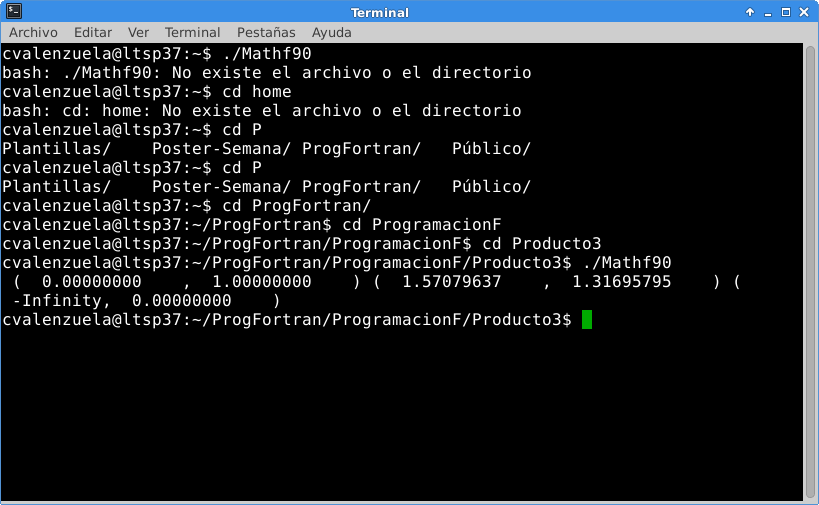
\includegraphics[width=0.5cm]{Mathf90.png}\\
 \end{center}
 7.Función 1+sin\\
  Se corrigió la sintaxis para poder compilarlo correctamente, de tal manera que al declarar las variables x,y, la función nos arrojó los valores correspondientes de f(x,y)= 1+sin(x,y).\\
  \begin{verbatim}
 ! Function . f90 : Program calls a simple function
 ! −−−−−−−−−−−−−−−−−−−−−−−−−−−−−−−
 Real *8 Function f (x,y)
   Implicit None
   Real *8 :: x, y
   f = 1.0 + sin (x*y )
 End Function f
 !
 Program Main
  Implicit None
  Real *8 :: Xin =0.25 , Yin =2. , c , f ! declarations ( also f)
  c = f ( Xin , Yin )
  write ( * , * ) 'f(Xin, Yin) = ' , c
 End Program Main
 \end{verbatim}
  \begin{center}
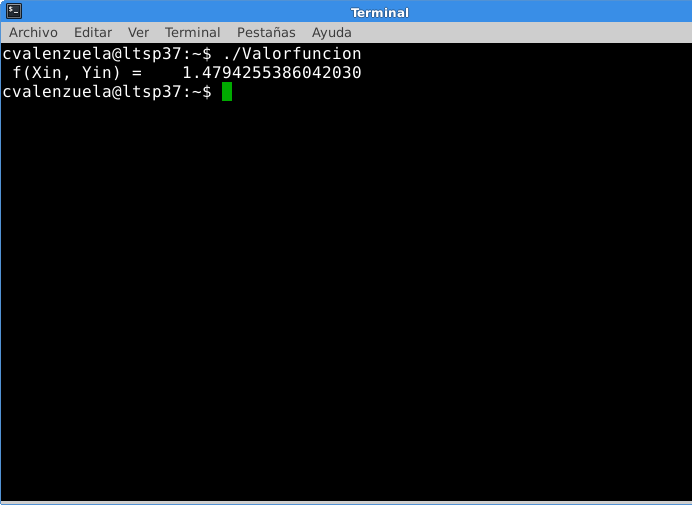
\includegraphics[width=0.5cm]{Valorfuncion.png}\\
 \end{center}
  8. Subrutinas.\\
  Se modificó la sintaxis para su correcta compilación y corrimiento. En realidad no presentó mayores dificultades.\\
  \begin{verbatim}
   ! Subroutine . f90 : Demonstrates the call for a simple subroutine
 ! −−−−−−−−−−−−−−−−−−−−−−−−−−−−−−−−−−−−−−−−−−−−−
 Subroutine g(x, y, ans1 , ans2 )
   Implicit None
   Real (8) :: x , y , ans1 , ans2 ! Declare variables
   ans1 = sin (x*y) + 1. ! Use sine intrinsic func.
   ans2 = ans1**2
 End Subroutine g
 !
 Program Mainprogram ! Demos the CALL
   Implicit None
   Real *8 :: Xin =0.25 , Yin =2.0 , Gout1 , Gout2
   call g( Xin , Yin , Gout1 , Gout2 ) ! Call the subr g
   write ( * , *) 'The answers are: ' , Gout1 , Gout2
End Program Mainprogram
   \end{verbatim}
    \begin{center}
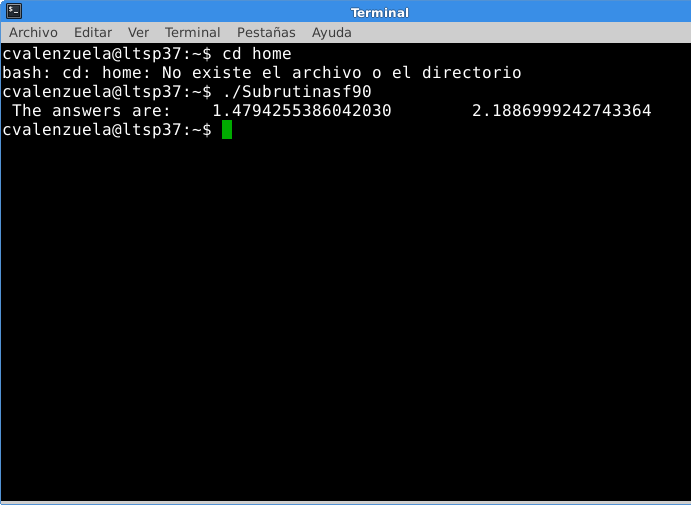
\includegraphics[width=0.5cm]{Subrutinas.png}\\
    \end{center}
  
  \end{document}